%%%%%%%%%%%%%%%%%%%%%%%%%%%%%%%%%%%%%%%%%
% Journal Article
% LaTeX Template
% Version 1.4 (15/5/16)
%
% This template has been downloaded from:
% http://www.LaTeXTemplates.com
%
% Original author:
% Frits Wenneker (http://www.howtotex.com) with extensive modifications by
% Vel (vel@LaTeXTemplates.com)
%
% License:
% CC BY-NC-SA 3.0 (http://creativecommons.org/licenses/by-nc-sa/3.0/)
%
%%%%%%%%%%%%%%%%%%%%%%%%%%%%%%%%%%%%%%%%%

%----------------------------------------------------------------------------------------
%	PACKAGES AND OTHER DOCUMENT CONFIGURATIONS
%----------------------------------------------------------------------------------------

\documentclass[twoside,twocolumn]{article}

\usepackage{blindtext} % Package to generate dummy text throughout this template 

\usepackage[sc]{mathpazo} % Use the Palatino font
\usepackage[T1]{fontenc} % Use 8-bit encoding that has 256 glyphs
\linespread{1.05} % Line spacing - Palatino needs more space between lines
\usepackage{microtype} % Slightly tweak font spacing for aesthetics

\usepackage[english]{babel} % Language hyphenation and typographical rules

\usepackage[hmarginratio=1:1,top=32mm,columnsep=20pt]{geometry} % Document margins
\usepackage[hang, small,labelfont=bf,up,textfont=it,up]{caption} % Custom captions under/above floats in tables or figures
\usepackage{booktabs} % Horizontal rules in tables

\usepackage{lettrine} % The lettrine is the first enlarged letter at the beginning of the text

\usepackage{enumitem} % Customized lists
\setlist[itemize]{noitemsep} % Make itemize lists more compact

\usepackage{abstract} % Allows abstract customization
\renewcommand{\abstractnamefont}{\normalfont\bfseries} % Set the "Abstract" text to bold
\renewcommand{\abstracttextfont}{\normalfont\small\itshape} % Set the abstract itself to small italic text

\usepackage{titlesec} % Allows customization of titles
\renewcommand\thesection{\Roman{section}} % Roman numerals for the sections
\renewcommand\thesubsection{\roman{subsection}} % roman numerals for subsections
\titleformat{\section}[block]{\large\scshape\centering}{\thesection.}{1em}{} % Change the look of the section titles
\titleformat{\subsection}[block]{\large}{\thesubsection.}{1em}{} % Change the look of the section titles

\usepackage{fancyhdr} % Headers and footers
\pagestyle{fancy} % All pages have headers and footers
\fancyhead{} % Blank out the default header
\fancyfoot{} % Blank out the default footer
\fancyhead[C]{Harvey Hughes $\bullet$ November 2018 $\bullet$ Emmanuel College} % Custom header text
\fancyfoot[RO,LE]{\thepage} % Custom footer text

\usepackage{titling} % Customizing the title section

\usepackage{hyperref} % For hyperlinks in the PDF

\usepackage{graphicx}
\graphicspath{ {images/} }

\newenvironment{reusefigure}[2][htbp]
  {\addtocounter{figure}{-1}%
   \renewcommand{\theHfigure}{dupe-fig}% If you're using hyperref
   \renewcommand{\thefigure}{\ref{#2}}% Figure counter is \ref
   \renewcommand{\addcontentsline}[3]{}% Avoid placing figure in LoF
   \begin{figure}[#1]}
  {\end{figure}}
\usepackage{wrapfig}
\usepackage{amsmath}
%----------------------------------------------------------------------------------------
%	TITLE SECTION
%----------------------------------------------------------------------------------------

\setlength{\droptitle}{-4\baselineskip} % Move the title up

\pretitle{\begin{center}\Huge\bfseries} % Article title formatting
\posttitle{\end{center}} % Article title closing formatting
\title{Flight Control 3F1 } % Article title
\author{%
\\
\textsc{Harvey Hughes} \\
\normalsize Emmanuel College \\ % Your institution
\normalsize Lab Date : 14/11/18 \\
\normalsize \href{mailto:hh458@cam.ac.uk}{hh458@cam.ac.uk} % Your email address
}
\date{\today} % Leave empty to omit a date
\renewcommand{\maketitlehookd}{%
\begin{abstract}
\noindent
\blindtext
\newline
\end{abstract}
}

%----------------------------------------------------------------------------------------

\begin{document}

% Print the title
\maketitle

%----------------------------------------------------------------------------------------
%	ARTICLE CONTENTS
%----------------------------------------------------------------------------------------

\section{Introduction}

\lettrine[nindent=0em,lines=3]{O}   
safafdasf
%------------------------------------------------


\section{Results and Discussion}
\subsection{2.0 Manual control}
\begin{figure}[h]
  \centering
    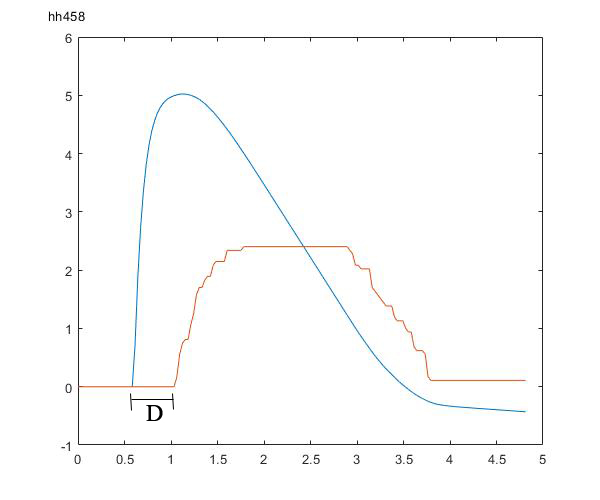
\includegraphics[width=\linewidth]{2_impulse}
  \caption{Typical response of manual control with a impulse disturbance of 5 }
  \label{fig:2impulse}
\end{figure}

\begin{figure}[h]
  \centering
    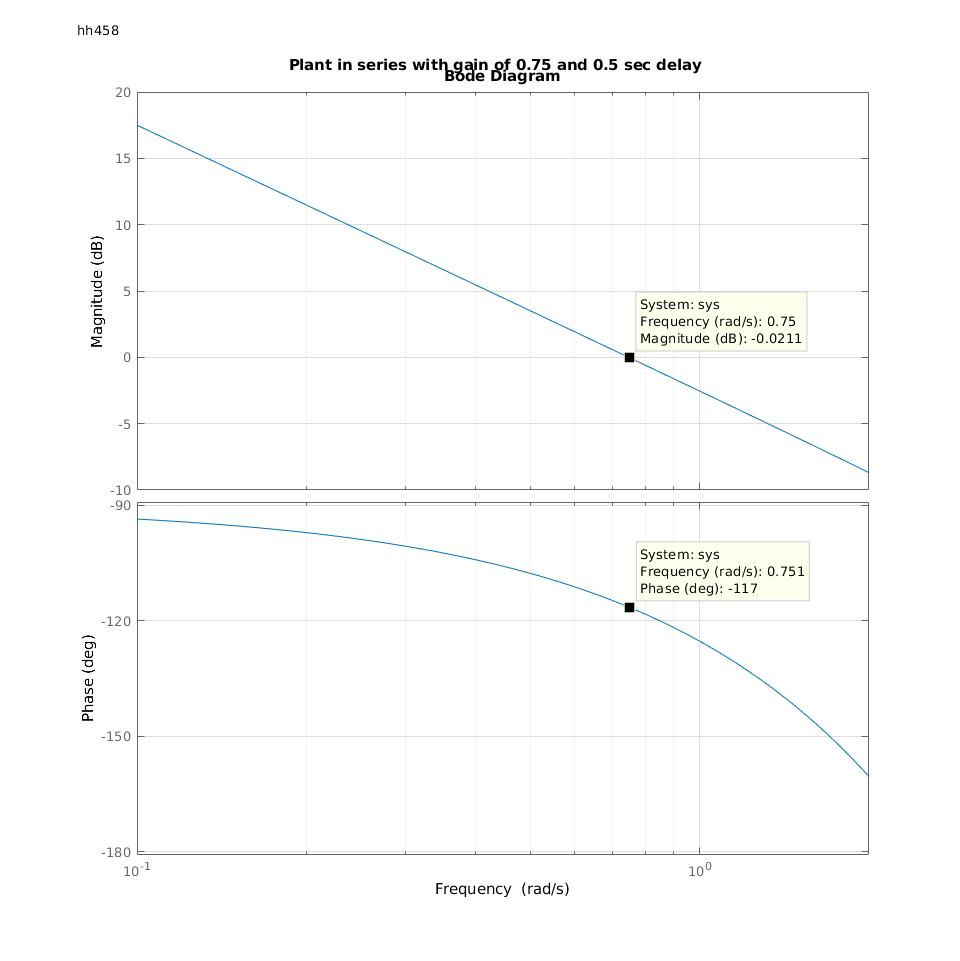
\includegraphics[width=\linewidth]{2_zoomed_in_bode}
  \caption{Bode plot of the controller with time delay 0.5 and gain 0.75 }
  \label{fig:2bode}
\end{figure}

\begin{equation}
\label{eq:manualmotion}
\begin{split}
&\ddot{y}(t) + M\dot{y}(t)=Nx(t)\\
& \overline{y}(s)=\frac{N}{s^2+Ms}\overline{x}(s)\\
&M=N=10\\
\end{split}
\end{equation}





The aircraft dynamics are modelled using equations \ref{eq:manualmotion} for this experiment. This experiment involves looking into the manual control of the aircraft and modelling our reactions as a controller. An impulse disturbance of magnitude 5 was tested first, the response for which can be seen in figure \ref{fig:2impulse}. From this graph you can estimate the time delay and gain that a manual controller has. The time delay was very constant across repeats and equalled D=0.5, the gain however varied between 0.5 (as pictured) and 1 across repeats so an average of k=0.75 was assumed for following calculations. This controller has a transfer function $ke^{-sD}$
\newline


\begin{figure}[h]
  \centering
    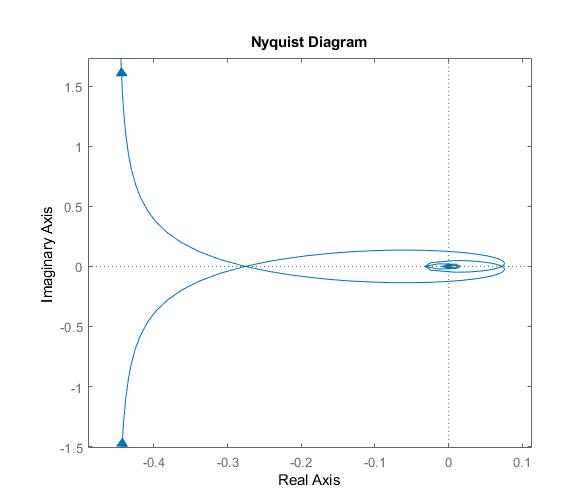
\includegraphics[width=\linewidth]{2_nyquist}
  \caption{Nyquist diagram sketch based off the response in figure \ref{fig:2bode} }
  \label{fig:2nyquist}
\end{figure}

Figure \ref{fig:2bode} shows the bode plot for the dynamics and controller of the plane. From this you can estimate the phase margin to be $180-117=63^{\circ}$ occurring at 0.75 rad/s. A time delay 'D' adds a phase shift of $\omega D$, therefore $63^{\circ}=1.1rad$ extra phase shift is possible and the time delay can be $\frac{1.1}{\omega}=\frac{1.1}{0.75}=1.47s$ longer. 
A sketch of the Nyquist diagram is shown in figure \ref{fig:2nyquist}.

\begin{figure}[h]
  \centering
    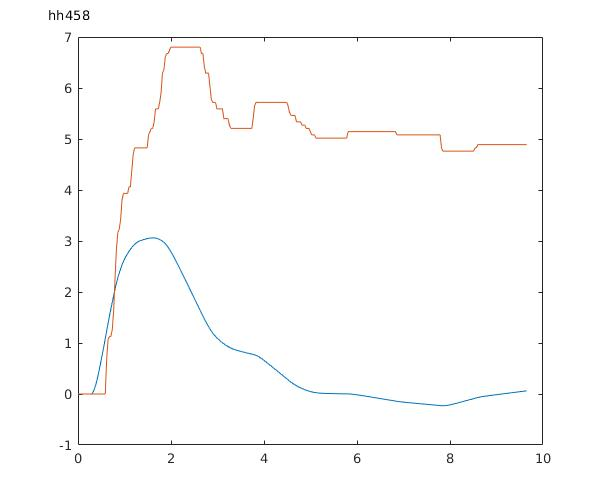
\includegraphics[width=\linewidth]{2_step}
  \caption{Typical response of manual control with a step disturbance of 5 }
  \label{fig:2step}
\end{figure}
A step disturbance of magnitude 5 was then tested. This is shown in figure \ref{fig:2step}. The goal was to keep the plane level throughout the flight. Integral action is present as steady state error can be observed to be tending to zero in figure \ref{fig:2step}, which is a characteristic of integral action. A non zero steady state error would cause the output to increase.
%-------------------------------------
\subsection{2.1 Pilot induced oscillation}
 \begin{figure}[h]
  \centering
    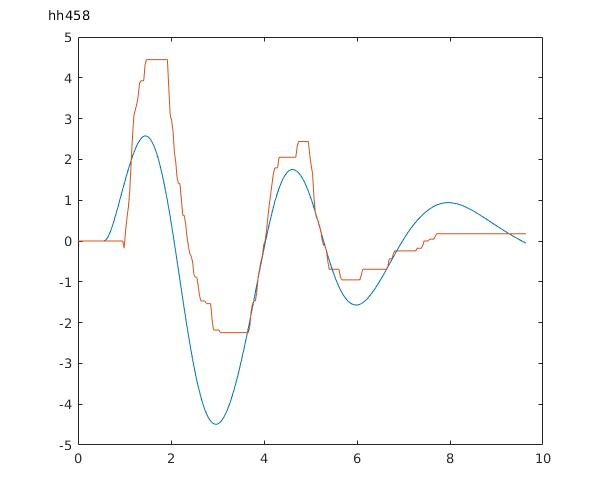
\includegraphics[width=\linewidth]{2-1_with_input}
  \caption{Typical response of pilot induced oscillations caused by attempting to stabilise the plane}
  \label{fig:2-1pio}
\end{figure}

\begin{equation}
\label{eq:pioeq}
\begin{split}
&G_1(s)=\frac{c}{(Ts+1)^3}\\
&T=\frac{4D}{\pi}\:\:c=\frac{\sqrt{8}}{k}\\
\end{split}
\end{equation}



 \begin{figure}[h]
  \centering
    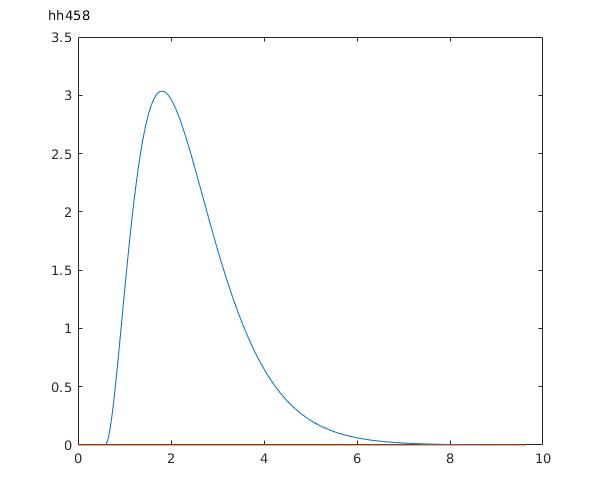
\includegraphics[width=\linewidth]{2-1_zero_input}
  \caption{Typical response of when no input is provided by the pilot, showing no oscillations}
  \label{fig:2-1zero}
\end{figure}

With an impulse disturbance of 5kD and an aircraft with transfer function in equation \ref{eq:pioeq} pilot induced oscillations can be observed. The typical response with pilot input is shown in figure \ref{fig:2-1pio} and shows a oscillation period of 3 seconds. Figure \ref{fig:2-1zero} shows the response when the pilot does nothing, and has not oscillatory response.
\newline

\begin{figure}[h]
  \centering
    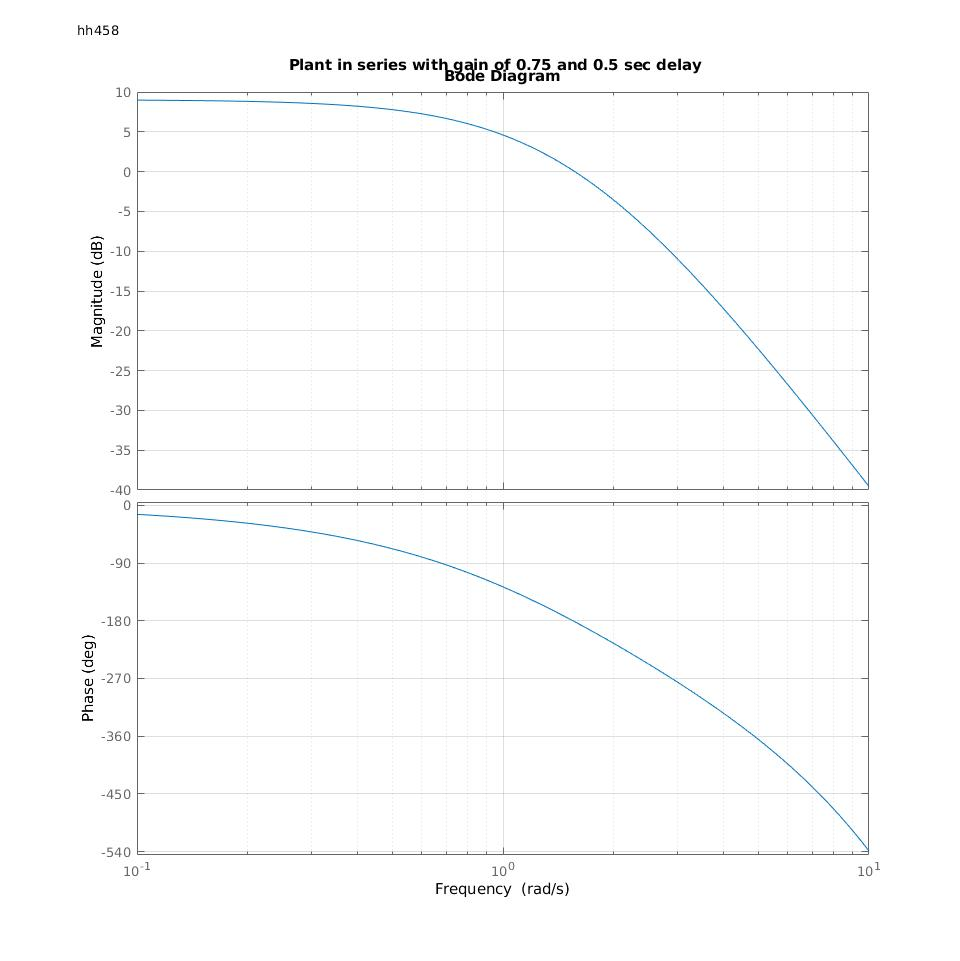
\includegraphics[width=\linewidth]{2-1_bode}
  \caption{Bode plot of the open loop response of the controller that caused PIO}
  \label{fig:2-1bode}
\end{figure}
Figure\ref{fig:2-1bode} shows the bode plot for this aircraft. Using this the oscillations can be explained as the gain is approximately 0dB when the phase is $-180^{\circ}$ and therefore has no phase margin. This 180 phase shift causes positive feedback of magnitude one and causes oscillations. The theoretical time period is calculated by $\omega = \frac{1}{T} =\frac{\pi}{2}, \: period = \frac{2\pi}{\omega}= 8D = 4s$ This is very similar to the observed result, with difference due to time delay during that experiment being faster then 0.5. Decreasing the time delay would increase the phase margin and help to solve this problem, additionally a controller with smaller gain would further help by introducing higher gain margin.
%-------------------------------------
\subsection{2.2 Sinusoidal disturbances}
\begin{figure}[h]
  \centering
    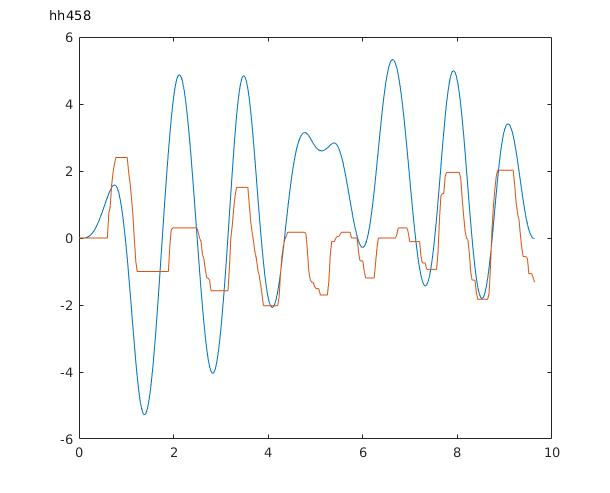
\includegraphics[width=\linewidth]{2-2}
  \caption{Typical response of attempting to stabilise a sinusoidal disturbance}
  \label{fig:2-2input}
\end{figure}

\begin{figure}[h]
  \centering
    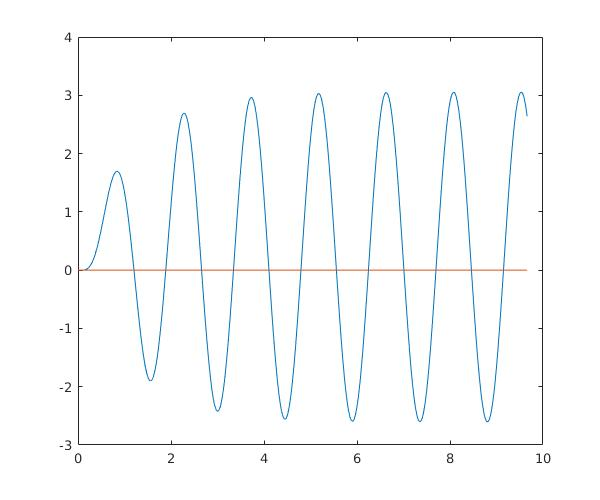
\includegraphics[width=\linewidth]{2-2-2}
  \caption{Typical response of a sinusoidal disturbance with no pilot input}
  \label{fig:2-2zero}
\end{figure}


\begin{figure}[h]
  \centering
    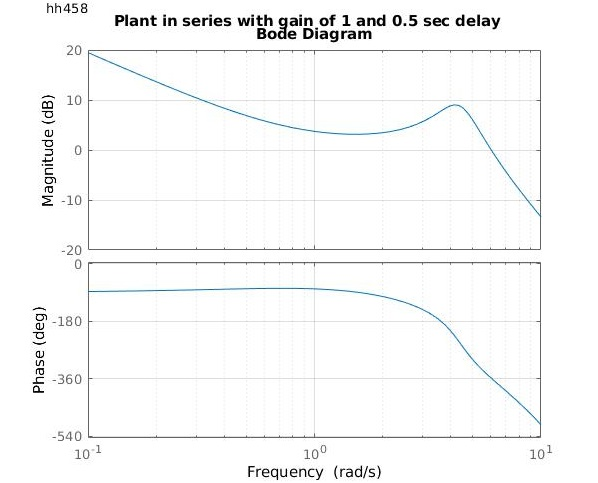
\includegraphics[width=\linewidth]{2-2_bode}
  \caption{Bode plot of the aircraft used for sinusoidal disturbances with gain 1 and delay 0.5}
  \label{fig:2-2bode}
\end{figure}

A sinusoidal disturbance of frequency 0.66Hz was tested on a F4E fighter aircraft, the typical response when trying to keep the plane level is shown in figure \ref{fig:2-2input}. With no pilot input the response is shown in figure \ref{fig:2-2input}, by comparing these two plots the error is observed to sometimes improve with a pilot input. However on average the error is the same or slightly worse than when no input is provided.

A bode plot is shown in figure \ref{fig:2-2bode} for this aircraft model using a controller of gain 1. When the phase is -180$^{\circ}$ the gain is 7.73dB therefore the maximum stable gain is $ 10^{-7.73/20}=0.4107$. The gain and phase at 0.66Hz=4.147rad/s is 9dB and -223$^{\circ}$ respectively. Upon implementing smaller movements (less controller gain) I was able to stabilize the aircraft better then initially.

The open and closed loop transfer functions between the aircraft position and disturbance are listed in equation \ref{eq:io}. These have been calculated using the block diagram located in the handout.

\begin{equation}
\label{eq:io}
\begin{split}
&Closed \: Loop: G(s)\\
&Open \: Loop: \frac{G(s)}{1+kG(s)}\\
\end{split}
\end{equation}

%-------------------------------------

\subsection{2.3 Unstable aircraft}
\begin{figure}[h]
  \centering
    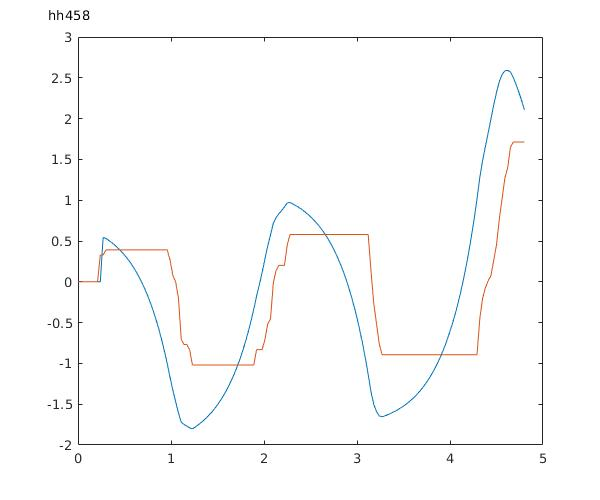
\includegraphics[width=\linewidth]{2-3_T=0-35}
  \caption{Response of stabilising the fastest pole in an unstable aircraft, with pole at T=0.35}
  \label{fig:2-3fastest}
\end{figure}


\begin{figure}[h]
  \centering
    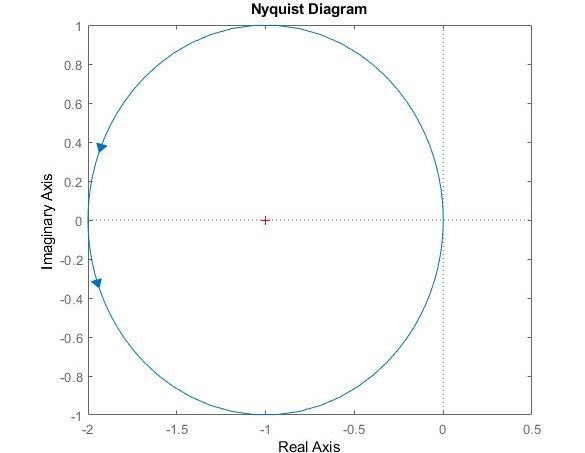
\includegraphics[width=\linewidth]{2-3_nyquist}
  \caption{Nyquist diagram for the unstable aircraft for T=1}
  \label{fig:2-3nyquist}
\end{figure}

\begin{figure}[h]
  \centering
    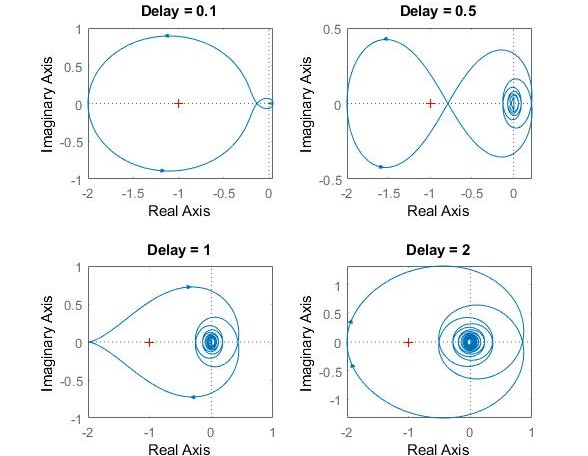
\includegraphics[width=\linewidth]{2-3_nyquist2}
  \caption{Nyquist diagram for the unstable aircraft for T=1 with four different time delays}
  \label{fig:2-3nyquist2}
\end{figure}

\begin{equation}
\label{eq:g2}
\begin{split}
&G_2(s) = \frac{2}{sT-1}\\
\end{split}
\end{equation}


An unstable aircraft with transfer function in equation \ref{eq:g2} was tested. The fastest pole that could be stabilised over a 5 second flight was T=0.35 and the response is plotted in figure \ref{fig:2-3fastest}. This pole is located at 1/T = 2.86.


The system is stable if the number of counter clockwise encirclements of the point -1/k is equal to the number of open loop poles in the right hand plane. The unstable aircraft has one unstable pole at 1/T therefore one encirclement is needed. The Nyquist diagram in figure \ref{fig:2-3nyquist} with gain 1 shows a crossing at -2=-1/0.5 therefore for any gain larger then 0.5 the system is stable. For a small time delay the Nyquist plot will encircle the origin, four time delays are plotted in figure \ref{fig:2-3nyquist2}. This delay can introduce instability as the point -1/k could get encircled clockwise.
%-------------------------------------

\subsection{3.0 Autopilot}
\begin{figure}[h]
  \centering
    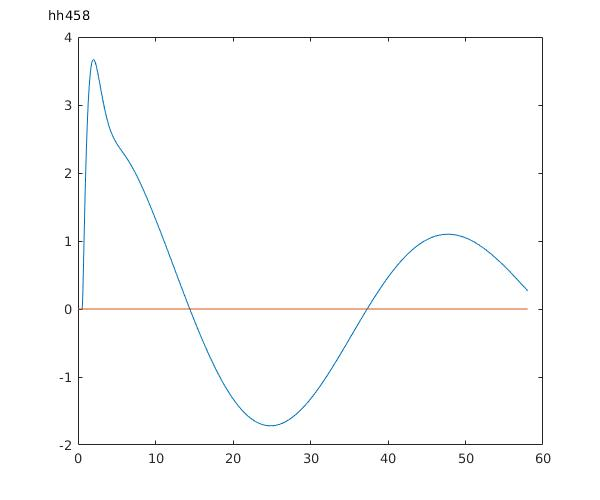
\includegraphics[width=\linewidth]{3_min_wait}
  \caption{Lightly damped phugoid motion due to impulse disturbance }
  \label{fig:3phugoid}
\end{figure}

\begin{figure}[h]
  \centering
    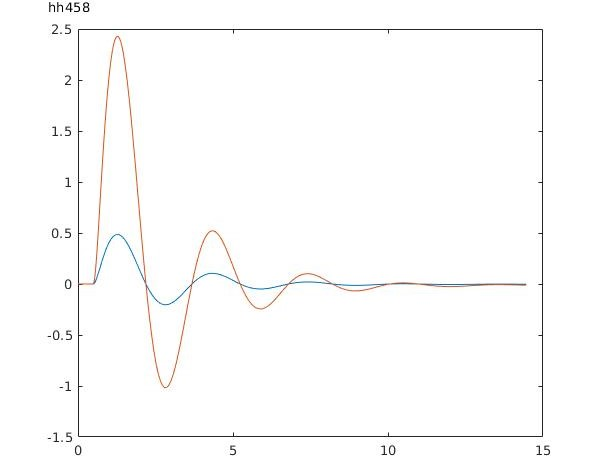
\includegraphics[width=\linewidth]{3_kp=5}
  \caption{Typical response when a proportional controller with gain 5 is implemented}
  \label{fig:3kp5}
\end{figure}

\begin{figure}[h]
  \centering
    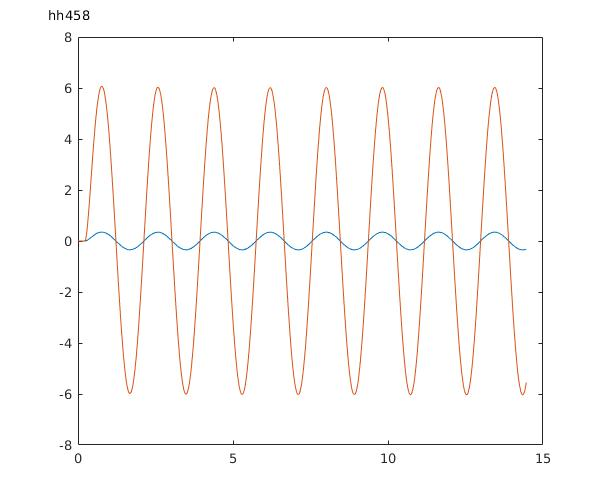
\includegraphics[width=\linewidth]{3_kp=17-4}
  \caption{Typical response when a proportional controller with gain 17.4 is implemented}
  \label{fig:3kp17-4}
\end{figure}

An aircraft with transfer function $G_3(s)$ from the handout was tested under an impulse disturbance, the response with no input is shown in figure \ref{fig:3phugoid}. This shows a lightly damped oscillation which is the phugoid mode of the aircraft. An initial auto pilot with proportional gain ($K_p$) 5 was then implemented to reduce this. The results are shown in figure \ref{fig:3-1first}. The proportional gain of 5 stabilised this oscillation. $K_p$ was increased to find the value at which oscillations remained stable with no decay, this is shown in figure \ref{fig:3-1increased} and occurred at a gain of 17.4. The observed oscillations have a period of 1.8 seconds. The gain margin with $k_p$ set to 5 is 12.4 as when gain is greater than 17.4 oscillations explode and the system is therefore unstable.
%-------------------------------------
\subsection{3.1 PID controller}
\begin{figure}[h]
  \centering
    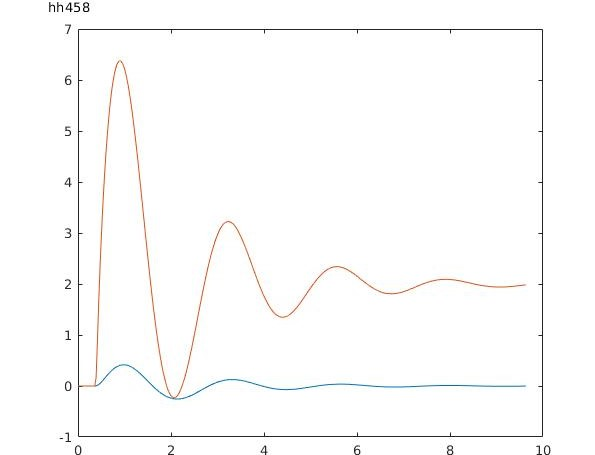
\includegraphics[width=\linewidth]{3-1_first_kd}
  \caption{Typical response when a PID controller is implemented with $K_p = 10.44,\:T_i=0.9,\:T_d=0.225$, the disturbance is an impulse and step of magnitude 2}
  \label{fig:3-1first}
\end{figure}

\begin{figure}[h]
  \centering
    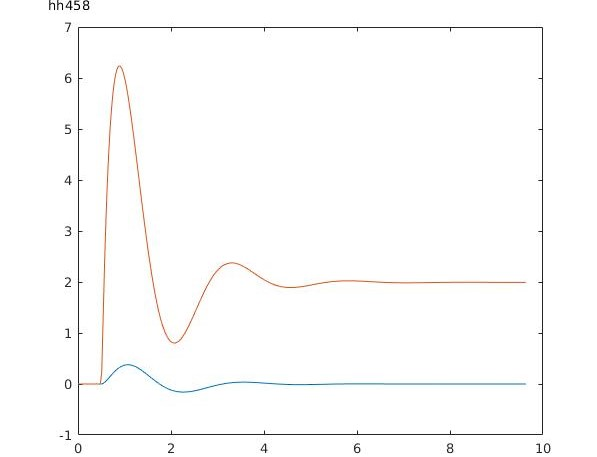
\includegraphics[width=\linewidth]{3-1_increased_kd}
  \caption{Typical response when a PID controller is implemented with $K_p = 10.44,\:T_i=0.9,\:T_d=0.315$ which is a 40\% increase to derivative gain, the disturbance is an impulse and step of magnitude 2}
  \label{fig:3-1increased}
\end{figure}

\begin{equation}
\label{eq:pid}
\begin{split}
&u(t) = K_p[e(t) + \frac{1}{T_i}\int_0^te(\tau)d\tau+T_d\frac{de}{dt}]\\
&\overline{u}(s)=K_p(1+\frac{1}{sT_i}+T_ds)\\
\end{split}
\end{equation}

A PID controller with transfer function in equation \ref{eq:pid} was implemented. $K_p,T_i \: and \: T_d$ took the values 10.44, 0.9 and 0.225 respectively. The response when using this controller is plotted in figure \ref{fig:3-1first}. The derivative gain was increased by 40\% with response shown in figure \ref{fig:3-1increased}. Increasing this gain has the effect of increasing damping of the oscillations.
%-------------------------------------
\subsection{3.2 Integrator wind-up}
\begin{figure}[h]
  \centering
    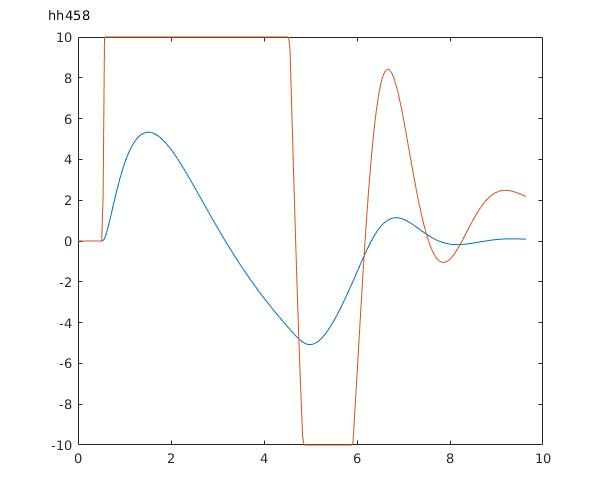
\includegraphics[width=\linewidth]{3-2_first_go}
  \caption{Typical response when a PID controller is implemented with $K_p = 10.44,\:T_i=0.9,\:T_d=0.315$, to a step disturbance of magnitude 2 and impulse magnitude 20}
  \label{fig:3-2first}
\end{figure}

\begin{figure}[h]
  \centering
    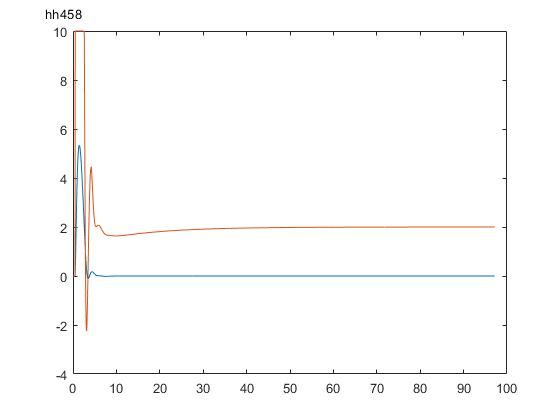
\includegraphics[width=\linewidth]{0-172}
  \caption{Zero steady state error when a cap of 0.172 is implemented}
  \label{fig:3-20-172}
\end{figure}

\begin{figure}[h]
  \centering
    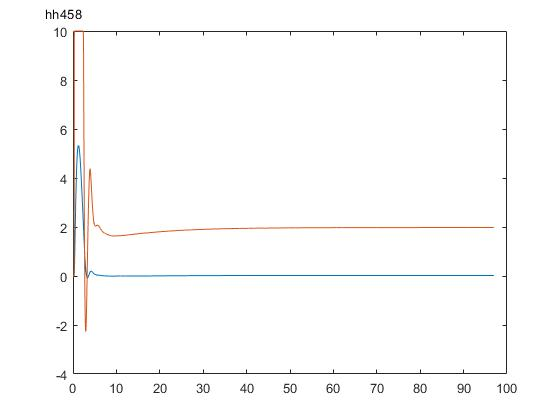
\includegraphics[width=\linewidth]{0-15sse0-022}
  \caption{Steady state error of 0.022 when a cap of 0.15 is implemented}
  \label{fig:3-20-15}
\end{figure}

\begin{equation}
\label{eq:iwu}
\begin{split}
&y(t=\infty)=\lim_{s\to 0}s\overline{y}(s)\\
&\overline{y}(s)=G_3(s)[\overline{u}(s)-\frac{2}{s}]\\ 
&No \: steady \: state \: error \: so \: y(t=\infty)=0\\
&0=\lim_{s\to 0}1.037[K_p(s+\frac{I_{min}}{T_i}+T_ds^2) -2]\\
&0=\frac{K_pI_{min}}{T_i}-2\\
&I_{min} = \frac{2T_i}{K_p} = 0.172\\
\end{split}
\end{equation}

Figure \ref{fig:3-2first} shows the response of this PID controller as before, there is an observed overshoot that causes the response to be oscillatory before settling down.
Unwanted overshoot can be caused if the integrator of the controller doesn't have a maximum value, this is called integrator wind up. A steady state error of zero exists when this cap is above 0.172 = $\frac{2T_i}{K_p}$. This is calculated in equation \ref{eq:iwu} and found by trial and error in Matlab and shown in figure \ref{fig:3-20-172}. Figure \ref{fig:3-20-15} shows the response when implementing a cap of 0.15 which is below the theoretical value, a steady state error of 0.022 was present.  
%-------------------------------------
%------------------------------------------------

\section{Conclusion}


%------------------------------------------------
\section{Appendix}


%------------------------------------------------
\end{document}
